\documentclass{standalone}

\usepackage[dvipsnames]{xcolor}
\usepackage{tikz}
\usetikzlibrary{arrows.meta}

\begin{document}
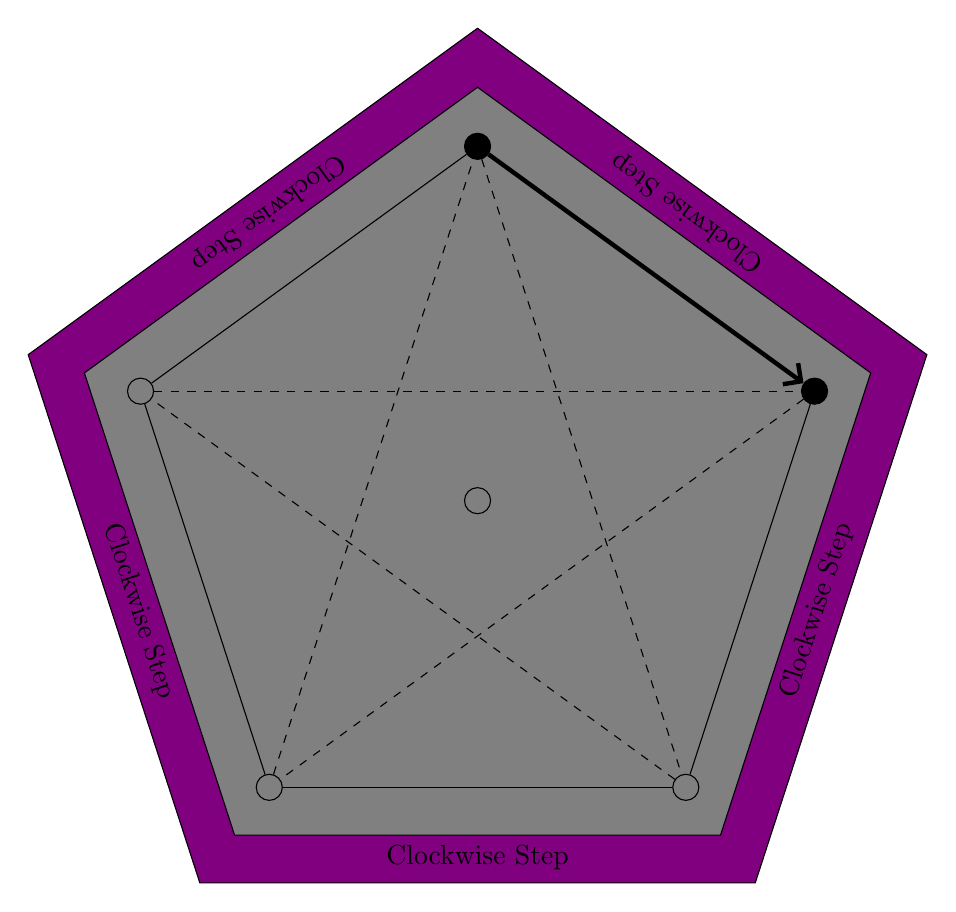
\begin{tikzpicture}
  \draw[fill=Purple] (90:6) -- (162:6) -- (234:6) -- (306:6) -- (18:6) -- cycle;
  \draw[fill=Gray] (90:5.25) -- (162:5.25) node[midway, below, sloped, rotate=180] {Clockwise Step}
                                            -- (234:5.25) node[midway, below, sloped] {Clockwise Step}
                                            -- (306:5.25) node[midway, below, sloped] {Clockwise Step}
                                            -- (18:5.25) node[midway, below, sloped] {Clockwise Step}
                                            -- cycle node[midway, below, sloped, rotate=180] {Clockwise Step};

  \node[draw, circle, fill=Black] (r) at (90:4.5) {};
  \node[draw, circle] (y) at (162:4.5) {};
  \node[draw, circle] (g) at (234:4.5) {};
  \node[draw, circle] (b) at (306:4.5) {};
  \node[draw, circle, fill=Black] (w) at (18:4.5) {};
  \node[draw, circle] (x) at (0,0) {};

  \draw[ultra thick, -{Straight Barb}] (r) -- (w);
  \draw (w) -- (b);
  \draw (b) -- (g);
  \draw (g) -- (y);
  \draw (y) -- (r);
  \draw[dashed] (r) -- (b);
  \draw[dashed] (b) -- (y);
  \draw[dashed] (y) -- (w);
  \draw[dashed] (w) -- (g);
  \draw[dashed] (g) -- (r);
\end{tikzpicture}

\end{document}